\documentclass{beamer}

%%%%%%%%%%%%%%%%%%%%%%%%%%%%%%%%%%%%% A MODIFIER %%%%%%%%%%%%%%%%%%%%%%%%%%%%%%%%%%%%%%%%%%%%%%
%%%%%%%%%%%%%%%%%%%%%%%%%%%%%%%%%%%%%%%%%%%%%%%%%%%%%%%%%%%%%%%%%%%%%%%%%%%%%%%%%%%%%%%%%%%%%%%

%%%%%%%%% Thème
\mode<presentation> {
	\usetheme{presentationleria}
}
%%%%%%%%%%%%%%%%%%%%%%%%%%%%%%%%%%%%%%%%%%%%%%%%%%%%%%%%%%%%%%%%%%%%%%%%%%%%%%%%%%%%%%%%%%%%%%%


%%%%%%%%% Packages obligatoires
\usepackage{lmodern}
\usepackage[T1]{fontenc}
\usepackage[utf8]{inputenc}
\usepackage[english]{babel}
\usepackage{graphicx}

\usepackage{tikz}
\usepackage{makecell}
% *******************************************************
% **** Tikz
% *******************************************************
\usetikzlibrary{trees}
\usetikzlibrary{shapes.geometric, arrows} % Flowchart
\usetikzlibrary{decorations.pathreplacing,calligraphy} % Curly braces

\tikzstyle{rectangleex} = [rectangle, minimum width=1cm, minimum height=0.4cm, draw=blue, fill=gray!75!black!10!bg]

\tikzstyle{arrow} = [thick,->,>=stealth, draw=red]

%%%%%%%%% Informations sur le document
\author[M. Legeay]{V. Barichard \and
C. Behuet \and
D. Genest \and
\textbf{M. Legeay} \and
D. Lesaint}
\institute[UnivAngers - LERIA]{UnivAngers - LERIA (France)\\\url{https://ua-usp.github.io/timetabling/}}
\titlegraphic{
  ~
  \hfill
  
\includegraphics[width=0.25\textwidth]{ua_h_couleur_ecran.png}
  \hfill
  
\includegraphics[width=0.25\textwidth]{logo_leria.pdf}
  \hfill
  ~
}

%%%%%%%%% Plan automatique
% Section
\AtBeginSection{\plansection}

% Sous-section
%\AtBeginSubsection{\plansoussection}

%%%%%%%%%%%%%%%%%%%%%%%%%%%%%%%%%%%%% A MODIFIER %%%%%%%%%%%%%%%%%%%%%%%%%%%%%%%%%%%%%%%%%%%%%%
%%%%%%%%%%%%%%%%%%%%%%%%%%%%%%%%%%%%%%%%%%%%%%%%%%%%%%%%%%%%%%%%%%%%%%%%%%%%%%%%%%%%%%%%%%%%%%%

%%%%%%%%%% Informations sur le document
% Titre :
\title[A Constraint Language for UTP]{Approche par contraintes pour une classe d'emplois du temps universitaires}
\subtitle{13th International Conference on the Practice and Theory of Automated Timetabling}
% Date (\today ou une date) :
\date{Leuven, Belgium | Tue 30 Aug 2022 – Fri 2 Sep 2022}
% Nom à affiche pour le plan (Plan, Sommaire, etc.) :
\newcommand{\nomplan}{Outline}

%%%%%%%%%% Packages additionnels


%%%%%%%%%% Commandes additionnels
\usepackage{PATAT_commands}
\definecolor{vert}{rgb}{0,.5,0}
\definecolor{pourpre}{rgb}{0.5,0.1,0.4}
\DeclareMathSymbol{:}{\mathord}{operators}{"3A} % permet d'enlever les espaces autour de ":" ; \mathrel{:} pour avoir le comportement par défaut

%%%%%%%%%%%%%%%%%%%%%%%%%%%%%%%%%%%%%%%%%%%%%%%%%%%%%%%%%%%%%%%%%%%%%%%%%%%%%%%%%%%%%%%%%%%%%%%


%%%%%%%%%%%%%%%%%%%%%%%%%%%%%%%%%%% BEGIN DOCUMENT %%%%%%%%%%%%%%%%%%%%%%%%%%%%%%%%%%%%%%%%%%%%
%%%%%%%%%%%%%%%%%%%%%%%%%%%%%%%%%%%%%%%%%%%%%%%%%%%%%%%%%%%%%%%%%%%%%%%%%%%%%%%%%%%%%%%%%%%%%%%
\begin{document}

%%%%%%%%%% Page de titre
\begin{frame}[noframenumbering,plain]
\titlepage
\end{frame}

%%%%%%%%%% Plan
\plan

%%%%%%%%%% Début du contenu
\section{Introduction}

\begin{frame}{Workflow for course organization of French universities}
    \begin{center}
    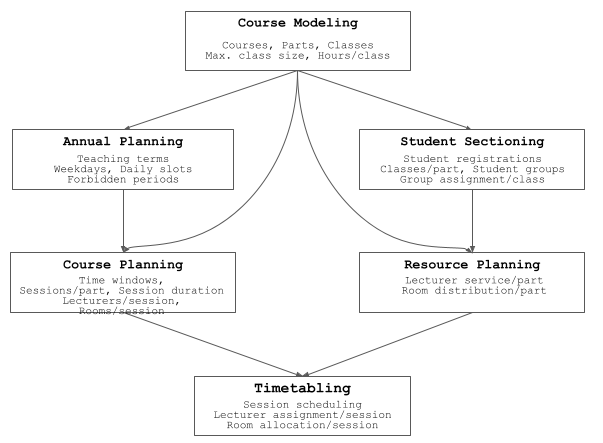
\includegraphics[scale=.38]{img/utp_workflow.png}
    \end{center}
    
    \begin{itemize}
        \item Students register to all the courses of a degree
        \item Lecturers must teach a certain amount of time
    \end{itemize}
\end{frame}

\begin{frame}{Timetabling problems}
\begin{minipage}{.49\textwidth}
    Related problems:
    \begin{itemize}
        \item curriculum balancing
        \item student sectioning
        \item examination timetabling
        \item curriculum-based timetabling
        \item tutor allocation
        \item timetabling perturbations
    \end{itemize}
\end{minipage}
\hfill
\begin{minipage}{.49\textwidth}
    Existing schemes:
    \begin{itemize}
        \item ITC-2007
        \item XHSST-2014
        \item ITC-2019
    \end{itemize}
    
    \vspace{1em}
    
    Solving methods:
    \begin{itemize}
        \item SAT
        \item ILP
        \item CP
        \item Metaheuristics
    \end{itemize}
\end{minipage}
\end{frame}

\begin{frame}{University Timetabling Problems (\UTP{})}
\framesubtitle{Our proposal}
\begin{minipage}{.43\textwidth}
    \begin{itemize}
        \item \UTP{}, a new class of problems: course scheduling, resource allocation and student sectioning
        \item \UTP{} language: \XML{}-based domain-specific language
    \end{itemize}
\end{minipage}
\hfill
\begin{minipage}{.55\textwidth}
\begin{center}
    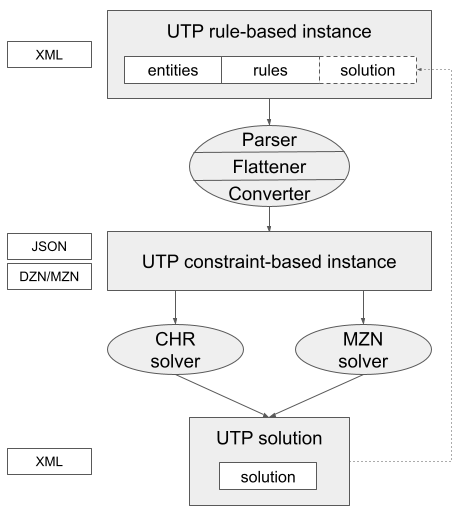
\includegraphics[scale=.38]{img/utp_toolchain.png}
\end{center}
\end{minipage}
\end{frame}

\section{\UTP{} language}
\subsection{Entity model}
\begin{frame}{Entity model}
    \begin{enumerate}
        \item Time horizon
        \item Course hierarchy
        \item Resource allocation
    \end{enumerate}
    \begin{center}
        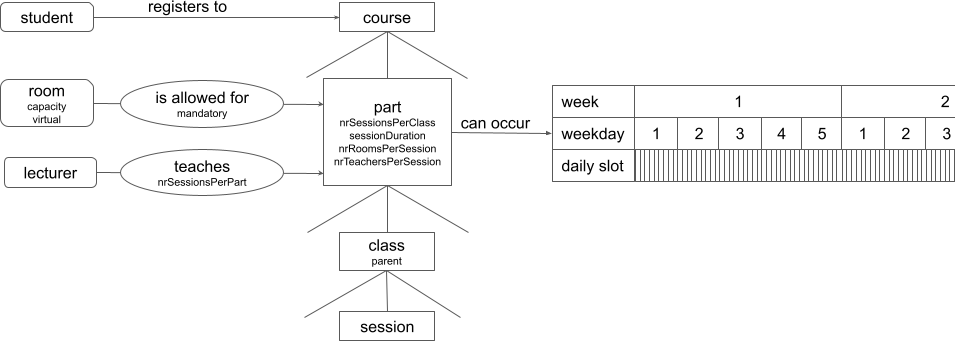
\includegraphics[width=\textwidth]{img/utp_entity_model.png}
    \end{center}
    \begin{itemize}
        \item Sessions ordered per class
    \end{itemize}
\end{frame}

\begin{frame}{Example}
    \begin{center}
    \only<1>{
        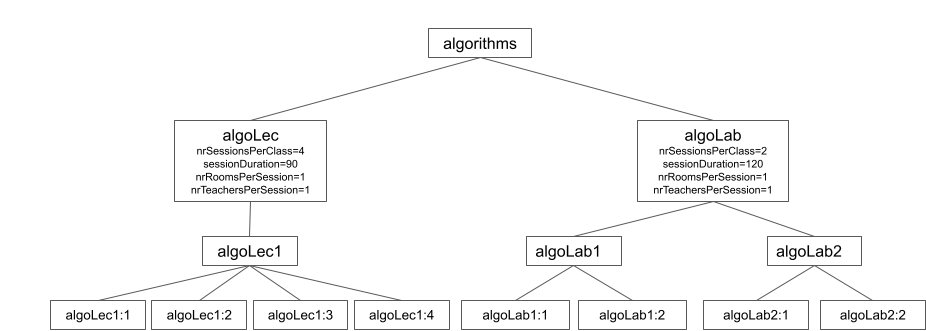
\includegraphics[width=\textwidth]{img/example_course-hierarchy.png}
    }
    \only<2>{
        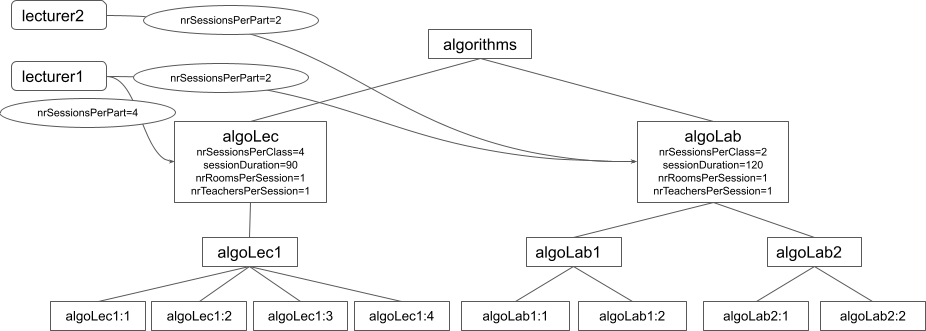
\includegraphics[width=\textwidth]{img/example_entity-model.png}
    }
    \end{center}
\end{frame}

\subsection{Constraints}
\begin{frame}{Constraints}
    \begin{itemize}
        \item Some constraints are built-in from the entity model
        \begin{itemize}
            \item resource pre-allocation (lecturers, rooms, students)
            \item session order
        \end{itemize}
        \item Definition of \UTP{} predicates
        \begin{itemize}
            \item \WEEKLY{}
            \item \SEQUENCED{}
            \item \SAMEROOMS{}
            \item \FORBIDDENPERIOD{}
            \item \ldots
        \end{itemize}
        \item Constraints can have parameters
        \item Constraints apply to sets of sessions linked to a resource (\textbf{e-maps})
    \end{itemize}
    
    \[predicate((\textcolor{red}{e_1},\textcolor{blue}{S_1}), \ldots,  (\textcolor{red}{e_m},\textcolor{blue}{S_m}), \textcolor{vert}{p_1}, \ldots, \textcolor{vert}{p_n})\]
\end{frame}

\begin{frame}{Examples}
    \begin{itemize}
        \item The first session of lab should start after the third lecture.
        \[{\SEQUENCED}((\textcolor{red}{algoLec1},\textcolor{blue}{\{algoLec1:3\}}), (\textcolor{red}{algoLab1},\textcolor{blue}{\{algoLab1:1\}}))\]
        \[{\SEQUENCED}((\textcolor{red}{algoLec1},\textcolor{blue}{\{algoLec1:3\}}), (\textcolor{red}{algoLab2},\textcolor{blue}{\{algoLab2:1\}}))\]
        \item lecturer2's lab sessions cannot occur on Tuesday of the 2nd week between 8am and 10am.
        \begin{flalign*} % "&" en début et fin de ligne pour aligner à gauche
        &{\FORBIDDENPERIOD}(&\\
        &(\textcolor{red}{lecturer2},\textcolor{blue}{\{algoLab1:1,algoLab1:2,algoLab2:1,algoLab2:2\}}),&\\
        &\textcolor{vert}{9120},\textcolor{vert}{9240})&
        \end{flalign*}
    \end{itemize}
\end{frame}

\subsection{Rules}
\begin{frame}{Rules}
    \begin{itemize}
        \item Rules generate constraints
        \item To create an e-map, rules use \textbf{selectors}: a generator and a optional list of filters $(\textcolor{pourpre}{T},\textcolor{orange}{L},\textcolor{brown}{O})$
        \begin{itemize}
            \item \textcolor{pourpre}{$T$}: entity type (lecturer $\TEACHER{}$, room $\ROOM{}$, student $\STUDENT{}$, courses $\COURSES{}$, course $\COURSE{}$, part $\PART{}$, class $\CLASS{}$)
            \item \textcolor{orange}{$L$}: label or identifier - optional
            \item \textcolor{brown}{$O$}: session ranks (mask) - optional
        \end{itemize}
        \item A rule is a predicate, a set of sets of selectors ($F_i$), and parameters
        \[predicate(F_1, \ldots, F_m, \textcolor{vert}{p_1}, \ldots, \textcolor{vert}{p_n})\]
        Where $F_i$ is denoted $\langle(\textcolor{pourpre}{T_1},\textcolor{orange}{L_1},\textcolor{brown}{O_1}), \ldots, (\textcolor{pourpre}{T_x},\textcolor{orange}{L_x},\textcolor{brown}{O_x}) \rangle$
        
        \item[] $(\textcolor{pourpre}{T_1},\textcolor{orange}{L_1},\textcolor{brown}{O_1})$ is the generator
        \item[] $(\textcolor{pourpre}{T_2},\textcolor{orange}{L_2},\textcolor{brown}{O_2}), \ldots, (\textcolor{pourpre}{T_x},\textcolor{orange}{L_x},\textcolor{brown}{O_x})$ are the filters
    \end{itemize}
\end{frame}

\begin{frame}{Examples}
    \begin{itemize}
        \item The first session of lab should start after the third lecture.
        \begin{flalign*}
        {\SEQUENCED}(&<(\textcolor{pourpre}{\CLASS},\textcolor{orange}{\_},\textcolor{brown}{\myset{3}}),(\textcolor{pourpre}{\PART},\textcolor{orange}{algoLec},\textcolor{brown}{\_})>,&\\
        &<(\textcolor{pourpre}{\CLASS},\textcolor{orange}{\_},\textcolor{brown}{\myset{1}}),(\textcolor{pourpre}{\PART},\textcolor{orange}{algoLab},\textcolor{brown}{\_})>)&\\
        \end{flalign*}
        
        \item lecturer2's lab sessions cannot occur on Tuesday of the 2nd week between 8am and 10am.
        \begin{flalign*}
        &{\FORBIDDENPERIOD}(<(\textcolor{pourpre}{\TEACHER},\textcolor{orange}{lecturer2},\textcolor{brown}{\_})>,\textcolor{vert}{9120},\textcolor{vert}{9240})&
        \end{flalign*}
    \end{itemize}
\end{frame}

\begin{frame}{Rules flattening}
    \begin{itemize}
        \item The \textit{generator} of the rule generates e-maps according to the type, identifier, and ranks of the generator and its filters
        \item All empty e-maps are removed
        \item A generator can generate several e-maps, the Cartesian product is applied in order to create the constraints
        \item The entity defined by the generator is used as the entity of the e-map
    \end{itemize}
\end{frame}

\begin{frame}{Rules flattening - \SEQUENCED{} example}
	\begin{tikzpicture}[]
        \node (A) [] {%
        $${\SEQUENCED}(\textbf<2-4>{<(\textcolor{pourpre}{\CLASS},\textcolor{orange}{\_},\textcolor{brown}{\myset{3}}),(\textcolor{pourpre}{\PART},\textcolor{orange}{algoLec},\textcolor{brown}{\_})>},$$%
        };
        \node (B) [below of=A, yshift=0.4cm, xshift=0.9cm] {%
        $$\textbf<5-8>{<(\textcolor{pourpre}{\CLASS},\textcolor{orange}{\_},\textcolor{brown}{\myset{1}}),(\textcolor{pourpre}{\PART},\textcolor{orange}{algoLab},\textcolor{brown}{\_})>})$$%
        };
        \visible<4->{\node (C) [rectangleex, xshift=5.5cm, yshift=0.2cm, right of=A] {%
        $$\{(\textcolor{red}{algoLec1},\textcolor{blue}{\{algoLec1:3\}})\}$$%
        };}
        \visible<8->{\node (D) [rectangleex, xshift=4.6cm, yshift=-0.2cm, right of=B] {\makecell[l]{%
        $$\{(\textcolor{red}{algoLab1},\textcolor{blue}{\{algoLab1:1\}}),$$\\
        $$(\textcolor{red}{algoLab2},\textcolor{blue}{\{algoLab2:1\}})\}$$}
        };}
        \visible<4->{\draw [arrow] (A) -- (C);}
        \visible<8->{\draw [arrow] (B.south) to[bend right] (D);}
    \end{tikzpicture}
    
    \begin{center}
        \only<1-2>{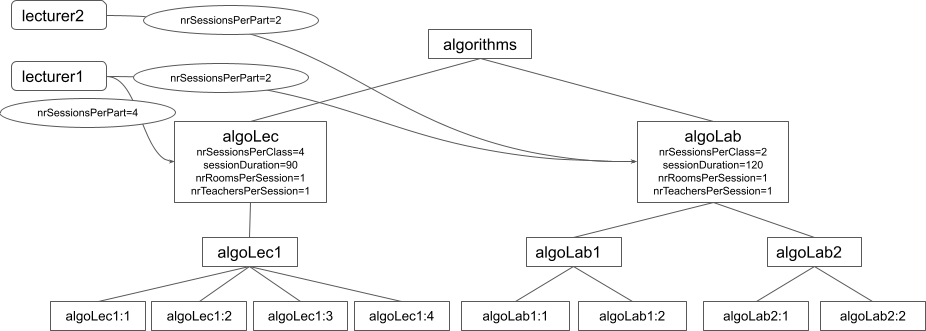
\includegraphics[width=\textwidth]{img/example_entity-model.png}}
        \only<3>{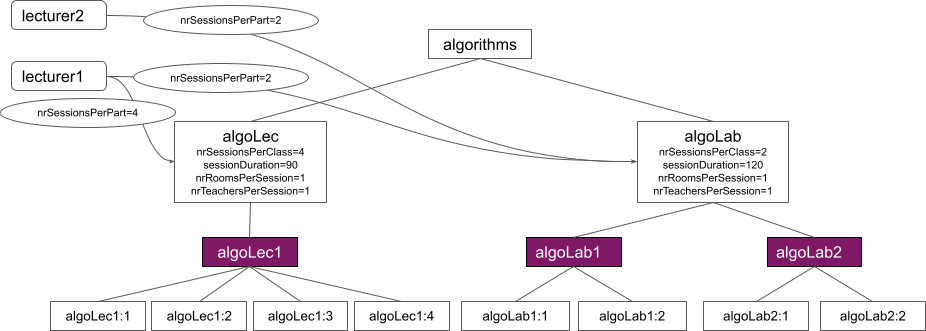
\includegraphics[width=\textwidth]{img/example_rule-flat_class.png}}
        \only<4>{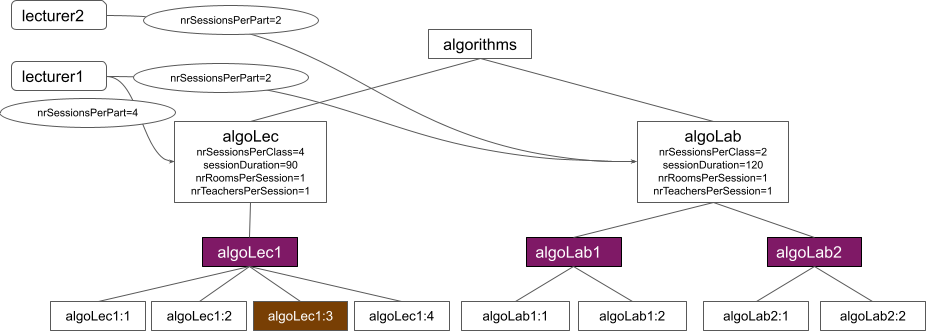
\includegraphics[width=\textwidth]{img/example_rule-flat_ses3.png}}
        \only<5>{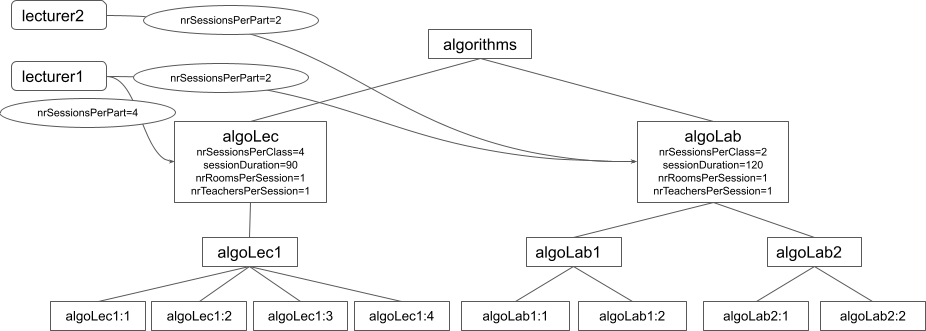
\includegraphics[width=\textwidth]{img/example_entity-model.png}}
        \only<6>{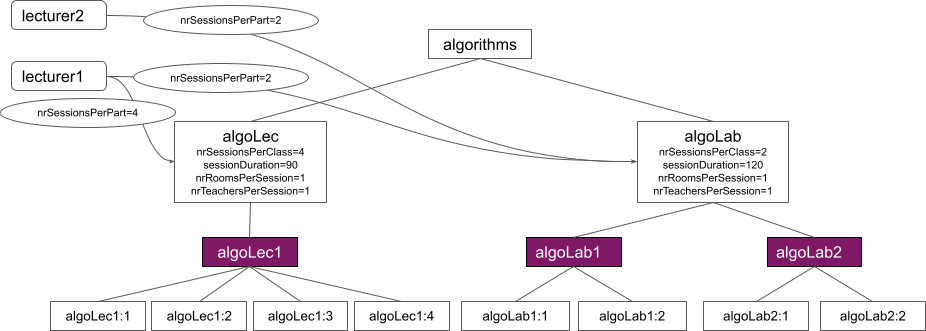
\includegraphics[width=\textwidth]{img/example_rule-flat_class.png}}
        \only<7>{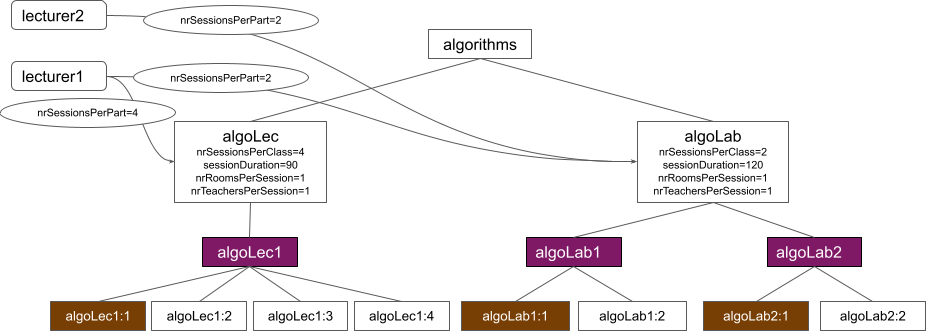
\includegraphics[width=\textwidth]{img/example_rule-flat_ses1.png}}
        \only<8>{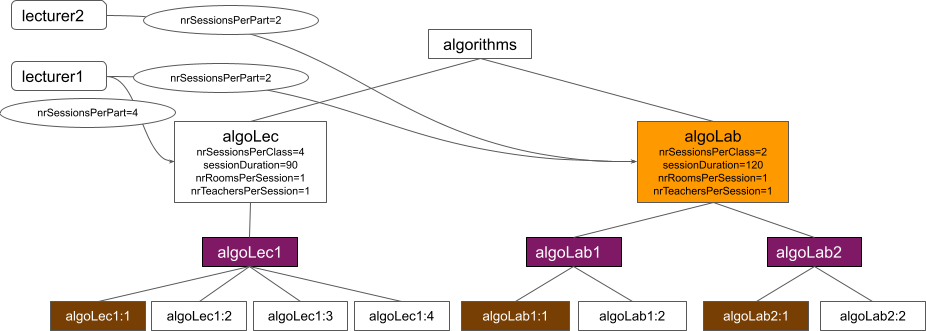
\includegraphics[width=\textwidth]{img/example_rule-flat_filter.png}}
        \only<9>{\[{\SEQUENCED}((\textcolor{red}{algoLec1},\textcolor{blue}{\{algoLec1:3\}}), (\textcolor{red}{algoLab1},\textcolor{blue}{\{algoLab1:1\}}))\]
        \[{\SEQUENCED}((\textcolor{red}{algoLec1},\textcolor{blue}{\{algoLec1:3\}}), (\textcolor{red}{algoLab2},\textcolor{blue}{\{algoLab2:1\}}))\]}
    \end{center}
\end{frame}

%\begin{frame}{Rules flattening - \SEQUENCED{} example}
%    \begin{flalign*}
%    {\SEQUENCED}(&\textbf<2-4>{<(\textcolor{pourpre}{\CLASS},\textcolor{orange}{\_},\textcolor{brown}{\myset{3}}),(\textcolor{pourpre}{\PART},\textcolor{orange}{algoLec},\textcolor{brown}{\_})>},&\only<4->{\{(\textcolor{red}{algoLec1},\textcolor{blue}{\{algoLec1:3\}})\}}\\
%    &\textbf<5-8>{<(\textcolor{pourpre}{\CLASS},\textcolor{orange}{\_},\textcolor{brown}{\myset{1}}),(\textcolor{pourpre}{\PART},\textcolor{orange}{algoLab},\textcolor{brown}{\_})>})&\only<8->{\{(\textcolor{red}{algoLab1},\textcolor{blue}{\{algoLab1:1\}}),}\\
%    &&\only<8->{(\textcolor{red}{algoLab2},\textcolor{blue}{\{algoLab2:1\}})\}}\\
%    \end{flalign*}
%    
%    \begin{center}
%        \only<1-2>{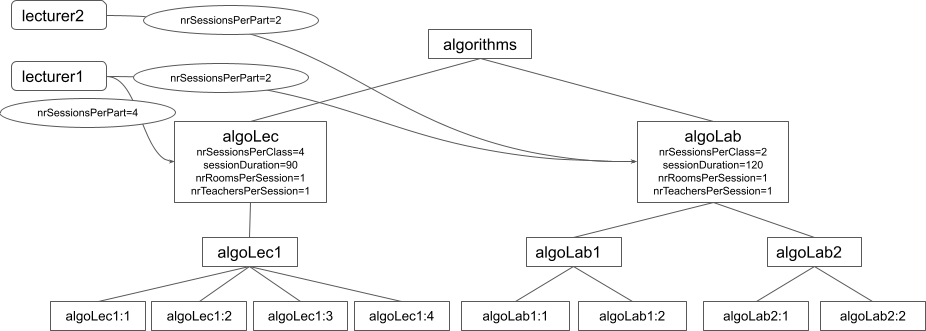
\includegraphics[width=\textwidth]{img/example_entity-model.png}}
%        \only<3>{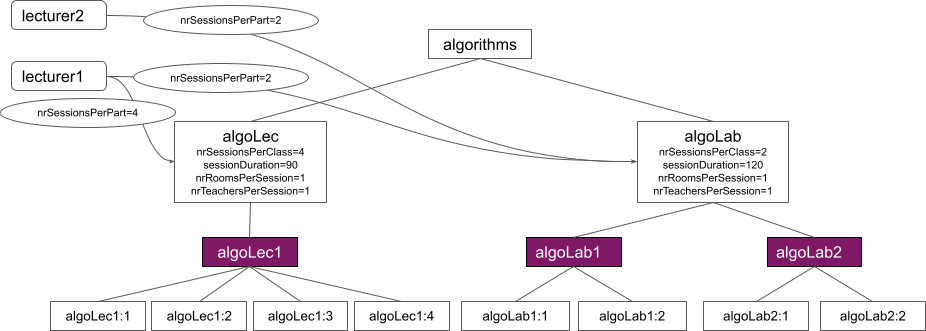
\includegraphics[width=\textwidth]{img/example_rule-flat_class.png}}
%        \only<4>{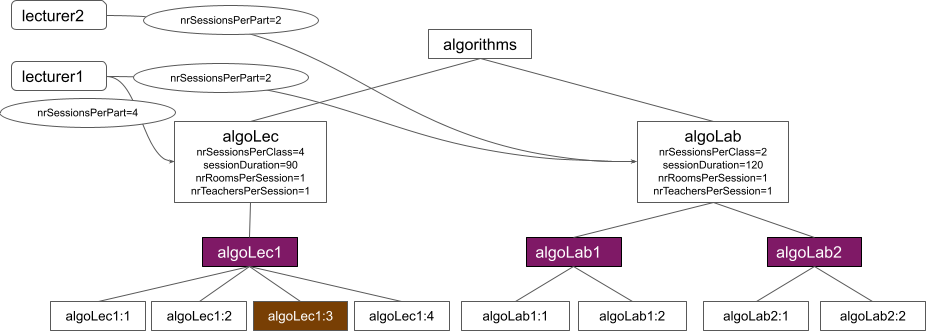
\includegraphics[width=\textwidth]{img/example_rule-flat_ses3.png}}
%        \only<5>{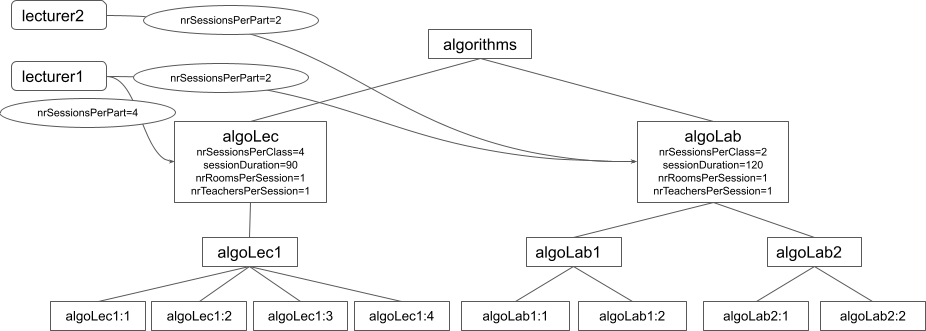
\includegraphics[width=\textwidth]{img/example_entity-model.png}}
%        \only<6>{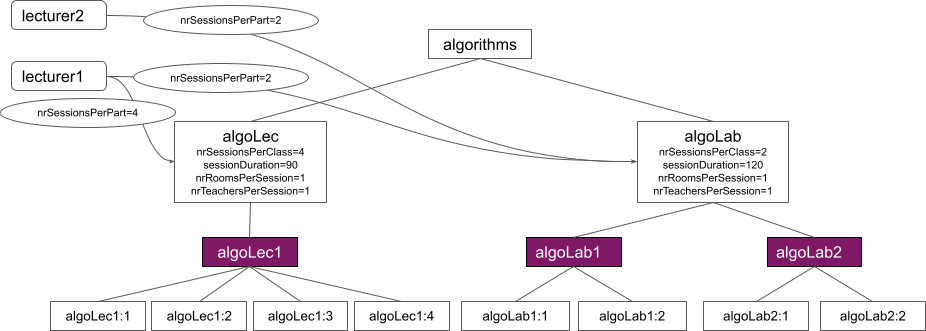
\includegraphics[width=\textwidth]{img/example_rule-flat_class.png}}
%        \only<7>{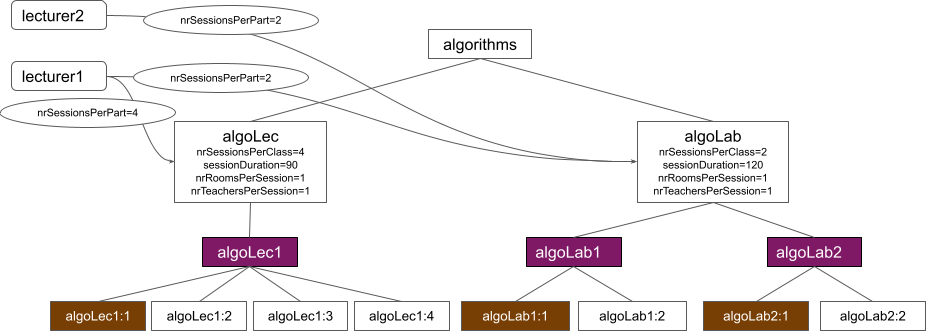
\includegraphics[width=\textwidth]{img/example_rule-flat_ses1.png}}
%        \only<8>{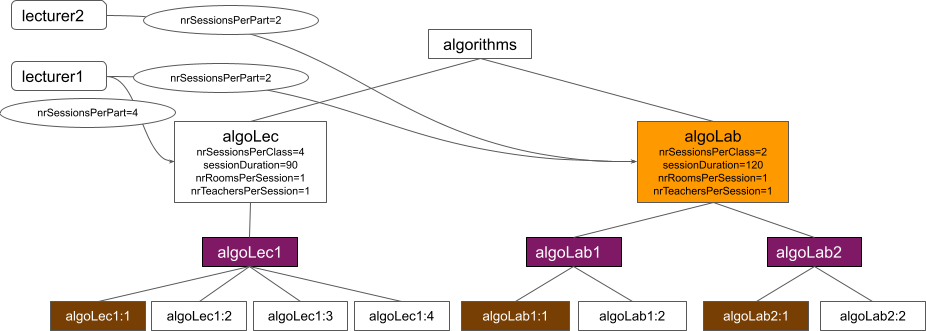
\includegraphics[width=\textwidth]{img/example_rule-flat_filter.png}}
%        \only<9>{\[{\SEQUENCED}((\textcolor{red}{algoLec1},\textcolor{blue}{\{algoLec1:3\}}), (\textcolor{red}{algoLab1},\textcolor{blue}{\{algoLab1:1\}}))\]
%        \[{\SEQUENCED}((\textcolor{red}{algoLec1},\textcolor{blue}{\{algoLec1:3\}}), (\textcolor{red}{algoLab2},\textcolor{blue}{\{algoLab2:1\}}))\]}
%    \end{center}
%\end{frame}

%\begin{frame}{Rules flattening - \FORBIDDENPERIOD{} example}
%    \begin{flalign*}
%    &{\FORBIDDENPERIOD}((<(\textcolor{pourpre}{\TEACHER},\textcolor{orange}{lecturer2},\textcolor{brown}{\_})>,\textcolor{vert}{9120},\textcolor{vert}{9240})&
%    \end{flalign*}
%    \begin{flalign*}
%    &&\only<4->{(\textcolor{red}{lecturer2},\textcolor{blue}{\{algoLab1:1,algoLab1:2,algoLab2:1,algoLab2:2\}})}
%    \end{flalign*}
%    
%    \begin{center}
%        \only<1>{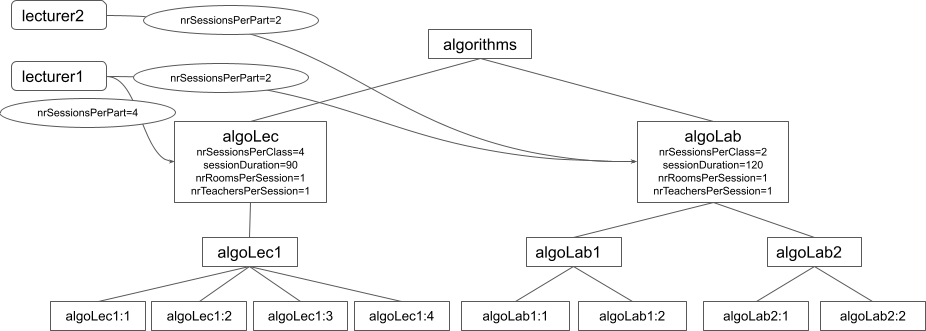
\includegraphics[width=\textwidth]{img/example_entity-model.png}}
%        \only<2>{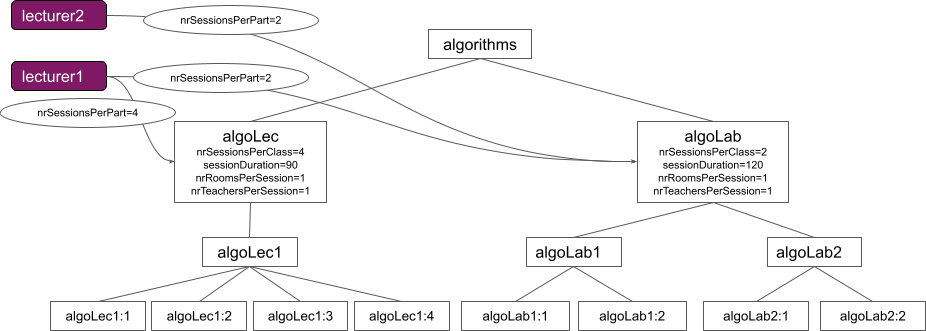
\includegraphics[width=\textwidth]{img/example_rule-flat_lecturers.png}}
%        \only<3>{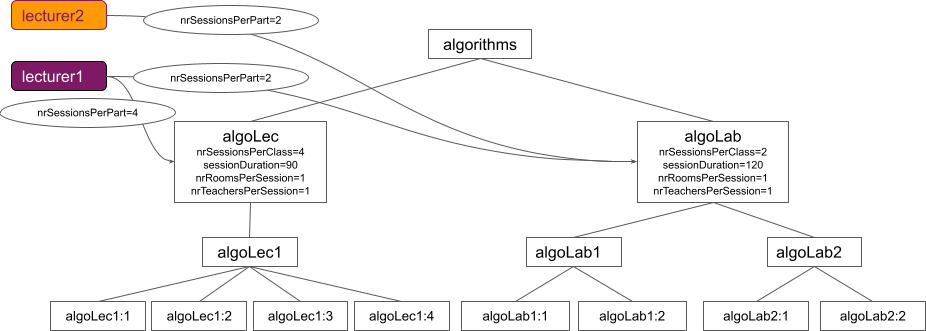
\includegraphics[width=\textwidth]{img/example_rule-flat_lecturer2.png}}
%        \only<4>{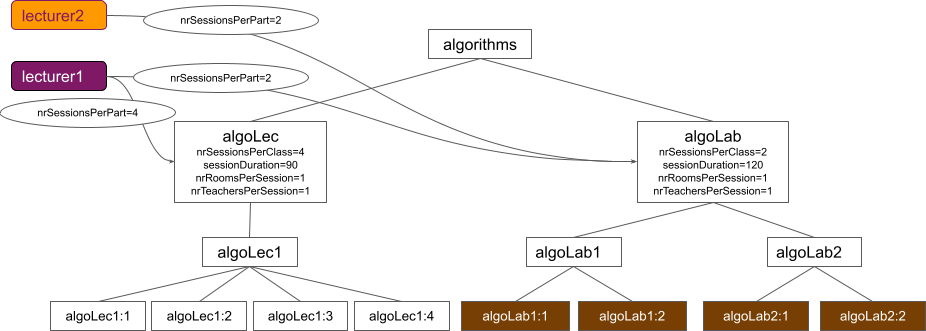
\includegraphics[width=\textwidth]{img/example_rule-flat_sesLab.png}}
%        \only<5>{\begin{flalign*} % "&" en début et fin de ligne pour aligner à gauche
%        &{\FORBIDDENPERIOD}(&\\
%        &(\textcolor{red}{lecturer2},\textcolor{blue}{\{algoLab1:1,algoLab1:2,algoLab2:1,algoLab2:2\}}),&\\
%        &\textcolor{vert}{9120},\textcolor{vert}{9240})&
%        \end{flalign*}}
%    \end{center}
%\end{frame}

\subsection{Solution}
\begin{frame}{Solution}
    \begin{itemize}
        \item Scheduling of resources ; assignment of students to groups ; assignment of groups to classes
        \item May be partial, empty, or inconsistent
        \begin{itemize}
            \item[$\Rightarrow$] enables support of subproblems (only scheduling, only sectioning, \ldots)
            \item[$\Rightarrow$] enables to repair an inconsistent solution
        \end{itemize}
    \end{itemize}
\end{frame}

\section{Model \& Implementation}
\begin{frame}{Model}
    We defined a Constraint Programming model with decision variables :
    \begin{itemize}
        \item students assigned to group (set variables)
        \item groups assigned to class (set variables)
        \item rooms assigned to session (set variables)
        \item lecturers assigned to session (set variables)
        \item starting slot assigned to session (integer variables)
    \end{itemize}
    And constraints expressed as built-in constraints or \UTP{} rules related to:
    \begin{itemize}
        \item student sectioning
        \item resource distribution
        \item session scheduling and resource allocation
    \end{itemize}
\end{frame}

\begin{frame}{Implementation}
    We developed 2 models leaving sectioning aside.
    
    \vfill
    
    \begin{minipage}[t]{.48\textwidth}
    \textbf{MiniZinc}
    \begin{itemize}
        \item Global constraints (disjunctive, cumulative)
        \item Strategy: rooms, lecturers then slots ; random choice for rooms and lecturers ; domain splitting for slots
    \end{itemize}
    \end{minipage}
    \hfill
    \begin{minipage}[t]{.48\textwidth}
    \textbf{Constraint Handling Rules}
    \begin{itemize}
        \item More decision variables
        \item Static and dynamic constraints (rules)
        \item Domain filtering
        \item Strategy: define the disjunctive graph of sessions
    \end{itemize}
    \end{minipage}
\end{frame}

\begin{frame}{Experiment}
    \begin{itemize}
        \item Real-life instance
        \item Bachelor in Computer sciences in UnivAngers
        \begin{itemize}
            \item 12 weeks, 5 days a week, 1440 slots per day (1 slot per minute)
            \item 9 courses, 25 parts, 48 classes, 262 sessions
            \item 67 students, 8 rooms, 12 lecturers
            \item 55 rules, 668 constraints
        \end{itemize}
        \item Solved in less than 5sec on both models
    \end{itemize}
\end{frame}

\section{Conclusion}

\begin{frame}{Conclusion}
    \begin{itemize}
        \item Introduction of a new class: University Timetable Problem (\UTP{})
        \item Introduction of a new language: \UTP{} language
        \item Work in progress
        \begin{itemize}
            \item Handle optimization
            \item Revise and repair
            \item More experiments with bigger real-life instances
        \end{itemize}
        \item Specifications, benchmarks and sources: \url{https://ua-usp.github.io/timetabling/}
    \end{itemize}
\end{frame}

%%%%%%%%%% Page de fin (page de titre)
\begin{frame}[noframenumbering,plain]
\titlepage
\end{frame}

\end{document}
